\documentclass[mathserif, 10pt]{beamer}
\usepackage{bm}
\usepackage{xspace}
\usepackage{amssymb}
\usepackage{amsmath}
\usepackage{amsfonts}
\usepackage{euscript}

\newcommand{\bba}{{\bf a}}
\newcommand{\bbb}{{\bf b}}
\newcommand{\bbc}{{\bf c}}
\newcommand{\bbd}{{\bf d}}
\newcommand{\bbe}{{\bf e}}
\newcommand{\bbf}{{\bf f}}
\newcommand{\bbg}{{\bf g}}
\newcommand{\bbh}{{\bf h}}
\newcommand{\bbi}{{\bf i}}
\newcommand{\bbj}{{\bf j}}
\newcommand{\bbk}{{\bf k}}
\newcommand{\bbl}{{\bf l}}
\newcommand{\bbm}{{\bf m}}
\newcommand{\bbn}{{\bf n}}
\newcommand{\bbo}{{\bf o}}
\newcommand{\bbp}{{\bf p}}
\newcommand{\bbq}{{\bf q}}
\newcommand{\bbr}{{\bf r}}
\newcommand{\bbs}{{\bf s}}
\newcommand{\bbt}{{\bf t}}
\newcommand{\bbu}{{\bf u}}
\newcommand{\bbv}{{\bf v}}
\newcommand{\bbx}{{\bf x}}
\newcommand{\bby}{{\bf y}}
\newcommand{\bbz}{{\bf z}}
\newcommand{\bbw}{{\bf w}}

\newcommand{\bbA}{{\bf A}}
\newcommand{\bbB}{{\bf B}}
\newcommand{\bbC}{{\bf C}}
\newcommand{\bbD}{{\bf D}}
\newcommand{\bbE}{{\bf E}}
\newcommand{\bbF}{{\bf F}}
\newcommand{\bbG}{{\bf G}}
\newcommand{\bbH}{{\bf H}}
\newcommand{\bbI}{{\bf I}}
\newcommand{\bbJ}{{\bf J}}
\newcommand{\bbK}{{\bf K}}
\newcommand{\bbL}{{\bf L}}
\newcommand{\bbM}{{\bf M}}
\newcommand{\bbN}{{\bf N}}
\newcommand{\bbO}{{\bf O}}
\newcommand{\bbP}{{\bf P}}
\newcommand{\bbQ}{{\bf Q}}
\newcommand{\bbR}{{\bf R}}
\newcommand{\bbS}{{\bf S}}
\newcommand{\bbT}{{\bf T}}
\newcommand{\bbU}{{\bf U}}
\newcommand{\bbV}{{\bf V}}
\newcommand{\bbX}{{\bf X}}
\newcommand{\bbZ}{{\bf Z}}
\newcommand{\bbY}{{\bf Y}}
\newcommand{\bbW}{{\bf W}}

\newcommand{\cca}{{\cal a}}
\newcommand{\ccb}{{\cal b}}
\newcommand{\ccc}{{\cal c}}
\newcommand{\ccd}{{\cal d}}
\newcommand{\cce}{{\cal e}}
\newcommand{\ccf}{{\cal f}}
\newcommand{\ccg}{{\cal g}}
\newcommand{\cch}{{\cal h}}
\newcommand{\cci}{{\cal i}}
\newcommand{\ccj}{{\cal j}}
\newcommand{\cck}{{\cal k}}
\newcommand{\ccl}{{\cal l}}
\newcommand{\ccm}{{\cal m}}
\newcommand{\ccn}{{\cal n}}
\newcommand{\cco}{{\cal o}}
\newcommand{\ccp}{{\cal p}}
\newcommand{\ccq}{{\cal q}}
\newcommand{\ccr}{{\cal r}}
\newcommand{\ccs}{{\cal s}}
\newcommand{\cct}{{\cal t}}
\newcommand{\ccu}{{\cal u}}
\newcommand{\ccv}{{\cal v}}
\newcommand{\ccx}{{\cal x}}
\newcommand{\ccy}{{\cal y}}
\newcommand{\ccz}{{\cal z}}
\newcommand{\ccw}{{\cal w}}

\newcommand{\ccA}{{\cal A}}
\newcommand{\ccB}{{\cal B}}
\newcommand{\ccC}{{\cal C}}
\newcommand{\ccD}{{\cal D}}
\newcommand{\ccE}{{\cal E}}
\newcommand{\ccF}{{\cal F}}
\newcommand{\ccG}{{\cal G}}
\newcommand{\ccH}{{\cal H}}
\newcommand{\ccI}{{\cal I}}
\newcommand{\ccJ}{{\cal J}}
\newcommand{\ccK}{{\cal K}}
\newcommand{\ccL}{{\cal L}}
\newcommand{\ccM}{{\cal M}}
\newcommand{\ccN}{{\cal N}}
\newcommand{\ccO}{{\cal O}}
\newcommand{\ccP}{{\cal P}}
\newcommand{\ccQ}{{\cal Q}}
\newcommand{\ccR}{{\cal R}}
\newcommand{\ccS}{{\cal S}}
\newcommand{\ccT}{{\cal T}}
\newcommand{\ccU}{{\cal U}}
\newcommand{\ccV}{{\cal V}}
\newcommand{\ccX}{{\cal X}}
\newcommand{\ccZ}{{\cal Z}}
\newcommand{\ccY}{{\cal Y}}
\newcommand{\ccW}{{\cal W}}

\newcommand{\bbwth}{\widetilde{\bf{h}}}
\newcommand{\bbwtx}{\widetilde{\bf{x}}}
\newcommand{\bbwtA}{\widetilde{\bf{A}}}
\newcommand{\bbwtH}{\widetilde{\bf{H}}}
\newcommand{\bbwtU}{\widetilde{\bf{U}}}
\newcommand{\bbwtS}{\widetilde{\bf{S}}}
\newcommand{\bbwtV}{\widetilde{\bf{V}}}

\newcommand{\BJ}{{\bf J}}
\newcommand{\mP}{{\mathcal P}}
\newcommand{\mU}{{\mathcal U}}
\newcommand{\mV}{{\mathcal V}}
\newcommand{\mX}{{\mathcal X}}
\newcommand{\rank}{{\mbox{rank}}}
\newcommand{\diag}{{\mbox{diag}}}
\newcommand{\kernel}{{\mbox{Ker}}}
\newcommand{\image}{{\mbox{Img}}}

\newcommand{\inv}{{-1}}

\newcommand{\bgamma}{\hbox{\boldmath $\gamma$}}
\newcommand{\bGamma}{\hbox{\boldmath $\Gamma$}}

\newcommand{\bnabla}{\hbox{\boldmath $\nabla$}}
%\newcommand{\bNabla}{\hbox{\boldmath $\Nabla$}}

\newcommand{\bups}{\hbox{\boldmath $\upsilon$}}
\newcommand{\bUps}{\hbox{\boldmath $\Upsilon$}}

\newcommand{\bomega}{\hbox{\boldmath $\omega$}}
\newcommand{\bOmega}{\hbox{\boldmath $\Omega$}}

\newcommand{\bpi}{\hbox{\boldmath $\pi$}}
\newcommand{\bPi}{\hbox{\boldmath $\Pi$}}

\newcommand{\bnu}{\hbox{\boldmath $\nu$}}
\newcommand{\bmu}{\hbox{\boldmath $\mu$}}

\newcommand{\sinc}{\mbox{sinc}}
\newcommand{\mbbZ}{{\mathbb Z}}
\newcommand{\mbbR}{{\mathbb R}}
\newcommand{\mbbP}{{\mathbb P}}

\newcommand{\bcX}{\hbox{\boldmath $\cal X$}}

\newcommand{\bzeta}{\hbox{\boldmath $\zeta$}}

\newcommand{\bxi}{\hbox{\boldmath $\xi$}}
\newcommand{\bchi}{\hbox{\boldmath $\chi$}}

\newcommand{\brho}{\hbox{\boldmath $\rho$}}

\newcommand{\blambda}{\hbox{\boldmath $\lambda$}}

\newcommand{\bveps}{\hbox{\boldmath $\varepsilon$}}

\newcommand{\bphi}{\hbox{\boldmath $\phi$}}
\newcommand{\bPhi}{\hbox{\boldmath $\Phi$}}

\newcommand{\bdelta}{\hbox{\boldmath $\delta$}}
\newcommand{\bDelta}{\hbox{\boldmath $\Delta$}}

\newcommand{\bPsi}{\hbox{\boldmath $\Psi$}}


\newcommand{\bvphi}{\hbox{\boldmath $\varphi$}}
\newcommand{\btau}{\hbox{\boldmath $\tau$}}
\newcommand{\bsigma}{\hbox{\boldmath $\sigma$}}
\newcommand{\bbeta}{\hbox{\boldmath $\beta$}}

%\renewcommand{\subfigcapskip}{1pt}
%\renewcommand{\subfigbottomskip}{1pt}

\newtheorem{Proposition}{\bf Proposition}
%\newtheorem{Theorem}{Theorem}
%\newtheorem{lemma}{Lemma}
%\newtheorem{theorproof}{Proof}

\newtheorem{propopreuve}{{\bf Preuve de la proposition}}
%\theoremstyle{break} 
\newtheorem{theoreme}{{\bf Th�or�me}}
\newtheorem{theorpreuve}{{\bf Preuve du th�or�me}}
\newtheorem{lemme}{{\bf Lemme}}
\newtheorem{lemmepreuve}{{\bf Preuve du lemme}}

\def\QED{\mbox{\rule[0pt]{1.5ex}{1.5ex}}}
\def\proof{\noindent\hspace{2em}{\it Proof: }}
%\def\endproof{\hspace*{\fill}~\QED\par\endtrivlist\unskip}
\def\endproof{\par}



\newcommand{\wha}{{\widehat a}}
\newcommand{\whb}{{\widehat b}}
\newcommand{\whc}{{\widehat c}}
\newcommand{\whd}{{\widehat d}}
\newcommand{\whe}{{\widehat e}}
\newcommand{\whf}{{\widehat f}}
\newcommand{\whg}{{\widehat g}}
\newcommand{\whh}{{\widehat h}}
\newcommand{\whi}{{\widehat i}}
\newcommand{\whj}{{\widehat j}}
\newcommand{\whk}{{\widehat k}}
\newcommand{\whl}{{\widehat l}}
\newcommand{\whm}{{\widehat m}}
\newcommand{\whn}{{\widehat n}}
\newcommand{\who}{{\widehat o}}
\newcommand{\whp}{{\widehat p}}
\newcommand{\whq}{{\widehat q}}
\newcommand{\whr}{{\widehat r}}
\newcommand{\whs}{{\widehat s}}
\newcommand{\wht}{{\widehat t}}
\newcommand{\whu}{{\widehat u}}
\newcommand{\whv}{{\widehat v}}
\newcommand{\whx}{{\widehat x}}
\newcommand{\why}{{\widehat y}}
\newcommand{\whz}{{\widehat z}}
\newcommand{\whw}{{\widehat w}}

\newcommand{\whA}{{\widehat A}}
\newcommand{\whB}{{\widehat B}}
\newcommand{\whC}{{\widehat C}}
\newcommand{\whD}{{\widehat D}}
\newcommand{\whE}{{\widehat E}}
\newcommand{\whF}{{\widehat F}}
\newcommand{\whG}{{\widehat G}}
\newcommand{\whH}{{\widehat H}}
\newcommand{\whI}{{\widehat I}}
\newcommand{\whJ}{{\widehat J}}
\newcommand{\whK}{{\widehat K}}
\newcommand{\whL}{{\widehat L}}
\newcommand{\whM}{{\widehat M}}
\newcommand{\whN}{{\widehat N}}
\newcommand{\whO}{{\widehat O}}
\newcommand{\whP}{{\widehat P}}
\newcommand{\whQ}{{\widehat Q}}
\newcommand{\whR}{{\widehat R}}
\newcommand{\whS}{{\widehat S}}
\newcommand{\whT}{{\widehat T}}
\newcommand{\whU}{{\widehat U}}
\newcommand{\whV}{{\widehat V}}
\newcommand{\whZ}{{\widehat X}}
\newcommand{\whY}{{\widehat Y}}
\newcommand{\whW}{{\widehat W}}

\newcommand{\whba}{{\widehat {\bf a}}}
\newcommand{\whbb}{{\widehat {\bf b}}}
\newcommand{\whbc}{{\widehat {\bf c}}}
\newcommand{\whbd}{{\widehat {\bf d}}}
\newcommand{\whbe}{{\widehat {\bf e}}}
\newcommand{\whbf}{{\widehat {\bf f}}}
\newcommand{\whbg}{{\widehat {\bf g}}}
\newcommand{\whbh}{{\widehat {\bf h}}}
\newcommand{\whbi}{{\widehat {\bf i}}}
\newcommand{\whbj}{{\widehat {\bf j}}}
\newcommand{\whbk}{{\widehat {\bf k}}}
\newcommand{\whbl}{{\widehat {\bf l}}}
\newcommand{\whbm}{{\widehat {\bf m}}}
\newcommand{\whbn}{{\widehat {\bf n}}}
\newcommand{\whbo}{{\widehat {\bf o}}}
\newcommand{\whbp}{{\widehat {\bf p}}}
\newcommand{\whbq}{{\widehat {\bf q}}}
\newcommand{\whbr}{{\widehat {\bf r}}}
\newcommand{\whbs}{{\widehat {\bf s}}}
\newcommand{\whbt}{{\widehat {\bf t}}}
\newcommand{\whbu}{{\widehat {\bf u}}}
\newcommand{\whbv}{{\widehat {\bf v}}}
\newcommand{\whbx}{{\widehat {\bf x}}}
\newcommand{\whby}{{\widehat {\bf y}}}
\newcommand{\whbz}{{\widehat {\bf z}}}
\newcommand{\whbw}{{\widehat {\bf w}}}

\newcommand{\whbA}{{\widehat {\bf A}}}
\newcommand{\whbB}{{\widehat {\bf B}}}
\newcommand{\whbC}{{\widehat {\bf C}}}
\newcommand{\whbD}{{\widehat {\bf D}}}
\newcommand{\whbE}{{\widehat {\bf E}}}
\newcommand{\whbF}{{\widehat {\bf F}}}
\newcommand{\whbG}{{\widehat {\bf G}}}
\newcommand{\whbH}{{\widehat {\bf H}}}
\newcommand{\whbI}{{\widehat {\bf I}}}
\newcommand{\whbJ}{{\widehat {\bf J}}}
\newcommand{\whbK}{{\widehat {\bf K}}}
\newcommand{\whbL}{{\widehat {\bf L}}}
\newcommand{\whbM}{{\widehat {\bf M}}}
\newcommand{\whbN}{{\widehat {\bf N}}}
\newcommand{\whbO}{{\widehat {\bf O}}}
\newcommand{\whbP}{{\widehat {\bf P}}}
\newcommand{\whbQ}{{\widehat {\bf Q}}}
\newcommand{\whbR}{{\widehat {\bf R}}}
\newcommand{\whbS}{{\widehat {\bf S}}}
\newcommand{\whbT}{{\widehat {\bf T}}}
\newcommand{\whbU}{{\widehat {\bf U}}}
\newcommand{\whbV}{{\widehat {\bf V}}}
\newcommand{\whbZ}{{\widehat {\bf X}}}
\newcommand{\whbY}{{\widehat {\bf Y}}}
\newcommand{\whbW}{{\widehat {\bf W}}}

\newcommand{\wta}{{\widetilde a}}
\newcommand{\wtb}{{\widetilde b}}
\newcommand{\wtc}{{\widetilde c}}
\newcommand{\wtd}{{\widetilde d}}
\newcommand{\wte}{{\widetilde e}}
\newcommand{\wtf}{{\widetilde f}}
\newcommand{\wtg}{{\widetilde g}}
\newcommand{\wth}{{\widetilde h}}
\newcommand{\wti}{{\widetilde i}}
\newcommand{\wtj}{{\widetilde j}}
\newcommand{\wtk}{{\widetilde k}}
\newcommand{\wtl}{{\widetilde l}}
\newcommand{\wtm}{{\widetilde m}}
\newcommand{\wtn}{{\widetilde n}}
\newcommand{\wto}{{\widetilde o}}
\newcommand{\wtp}{{\widetilde p}}
\newcommand{\wtq}{{\widetilde q}}
\newcommand{\wtr}{{\widetilde r}}
\newcommand{\wts}{{\widetilde s}}
\newcommand{\wtt}{{\widetilde t}}
\newcommand{\wtu}{{\widetilde u}}
\newcommand{\wtv}{{\widetilde v}}
\newcommand{\wtx}{{\widetilde x}}
\newcommand{\wty}{{\widetilde y}}
\newcommand{\wtz}{{\widetilde z}}
\newcommand{\wtw}{{\widetilde w}}

\newcommand{\wtA}{{\widetilde A}}
\newcommand{\wtB}{{\widetilde B}}
\newcommand{\wtC}{{\widetilde C}}
\newcommand{\wtD}{{\widetilde D}}
\newcommand{\wtE}{{\widetilde E}}
\newcommand{\wtF}{{\widetilde F}}
\newcommand{\wtG}{{\widetilde G}}
\newcommand{\wtH}{{\widetilde H}}
\newcommand{\wtI}{{\widetilde I}}
\newcommand{\wtJ}{{\widetilde J}}
\newcommand{\wtK}{{\widetilde K}}
\newcommand{\wtL}{{\widetilde L}}
\newcommand{\wtM}{{\widetilde M}}
\newcommand{\wtN}{{\widetilde N}}
\newcommand{\wtO}{{\widetilde O}}
\newcommand{\wtP}{{\widetilde P}}
\newcommand{\wtQ}{{\widetilde Q}}
\newcommand{\wtR}{{\widetilde R}}
\newcommand{\wtS}{{\widetilde S}}
\newcommand{\wtT}{{\widetilde T}}
\newcommand{\wtU}{{\widetilde U}}
\newcommand{\wtV}{{\widetilde V}}
\newcommand{\wtZ}{{\widetilde X}}
\newcommand{\wtY}{{\widetilde Y}}
\newcommand{\wtW}{{\widetilde W}}

\newcommand{\wtba}{{\widetilde {\bf a}}}
\newcommand{\wtbb}{{\widetilde {\bf b}}}
\newcommand{\wtbc}{{\widetilde {\bf c}}}
\newcommand{\wtbd}{{\widetilde {\bf d}}}
\newcommand{\wtbe}{{\widetilde {\bf e}}}
\newcommand{\wtbf}{{\widetilde {\bf f}}}
\newcommand{\wtbg}{{\widetilde {\bf g}}}
\newcommand{\wtbh}{{\widetilde {\bf h}}}
\newcommand{\wtbi}{{\widetilde {\bf i}}}
\newcommand{\wtbj}{{\widetilde {\bf j}}}
\newcommand{\wtbk}{{\widetilde {\bf k}}}
\newcommand{\wtbl}{{\widetilde {\bf l}}}
\newcommand{\wtbm}{{\widetilde {\bf m}}}
\newcommand{\wtbn}{{\widetilde {\bf n}}}
\newcommand{\wtbo}{{\widetilde {\bf o}}}
\newcommand{\wtbp}{{\widetilde {\bf p}}}
\newcommand{\wtbq}{{\widetilde {\bf q}}}
\newcommand{\wtbr}{{\widetilde {\bf r}}}
\newcommand{\wtbs}{{\widetilde {\bf s}}}
\newcommand{\wtbt}{{\widetilde {\bf t}}}
\newcommand{\wtbu}{{\widetilde {\bf u}}}
\newcommand{\wtbv}{{\widetilde {\bf v}}}
\newcommand{\wtbx}{{\widetilde {\bf x}}}
\newcommand{\wtby}{{\widetilde {\bf y}}}
\newcommand{\wtbz}{{\widetilde {\bf z}}}
\newcommand{\wtbw}{{\widetilde {\bf w}}}

\newcommand{\wtbA}{{\widetilde {\bf A}}}
\newcommand{\wtbB}{{\widetilde {\bf B}}}
\newcommand{\wtbC}{{\widetilde {\bf C}}}
\newcommand{\wtbD}{{\widetilde {\bf D}}}
\newcommand{\wtbE}{{\widetilde {\bf E}}}
\newcommand{\wtbF}{{\widetilde {\bf F}}}
\newcommand{\wtbG}{{\widetilde {\bf G}}}
\newcommand{\wtbH}{{\widetilde {\bf H}}}
\newcommand{\wtbI}{{\widetilde {\bf I}}}
\newcommand{\wtbJ}{{\widetilde {\bf J}}}
\newcommand{\wtbK}{{\widetilde {\bf K}}}
\newcommand{\wtbL}{{\widetilde {\bf L}}}
\newcommand{\wtbM}{{\widetilde {\bf M}}}
\newcommand{\wtbN}{{\widetilde {\bf N}}}
\newcommand{\wtbO}{{\widetilde {\bf O}}}
\newcommand{\wtbP}{{\widetilde {\bf P}}}
\newcommand{\wtbQ}{{\widetilde {\bf Q}}}
\newcommand{\wtbR}{{\widetilde {\bf R}}}
\newcommand{\wtbS}{{\widetilde {\bf S}}}
\newcommand{\wtbT}{{\widetilde {\bf T}}}
\newcommand{\wtbU}{{\widetilde {\bf U}}}
\newcommand{\wtbV}{{\widetilde {\bf V}}}
\newcommand{\wtbX}{{\widetilde {\bf X}}}
\newcommand{\wtbY}{{\widetilde {\bf Y}}}
\newcommand{\wtbW}{{\widetilde {\bf W}}}
\newcommand{\wtbcX}{{\widetilde {\boldmath $\cal X$}}}
\newcommand{\hx}{\hat{x}}
\newcommand{\hy}{\hat{y}}
\newcommand{\hw}{\hat{w}}


\def\olba {\ensuremath{{\overline {\bf a}}\xspace}}
\def\olbb {\ensuremath{{\overline {\bf b}}\xspace}}
\def\olbc {\ensuremath{{\overline {\bf c}}\xspace}}
\def\olbd {\ensuremath{{\overline {\bf d}}\xspace}}
\def\olbe {\ensuremath{{\overline {\bf e}}\xspace}}
\def\olbf {\ensuremath{{\overline {\bf f}}\xspace}}
\def\olbg {\ensuremath{{\overline {\bf g}}\xspace}}
\def\olbh {\ensuremath{{\overline {\bf h}}\xspace}}
\def\olbi {\ensuremath{{\overline {\bf i}}\xspace}}
\def\olbj {\ensuremath{{\overline {\bf j}}\xspace}}
\def\olbk {\ensuremath{{\overline {\bf k}}\xspace}}
\def\olbl {\ensuremath{{\overline {\bf l}}\xspace}}
\def\olbm {\ensuremath{{\overline {\bf m}}\xspace}}
\def\olbn {\ensuremath{{\overline {\bf n}}\xspace}}
\def\olbo {\ensuremath{{\overline {\bf o}}\xspace}}
\def\olbp {\ensuremath{{\overline {\bf p}}\xspace}}
\def\olbq {\ensuremath{{\overline {\bf q}}\xspace}}
\def\olbr {\ensuremath{{\overline {\bf r}}\xspace}}
\def\olbs {\ensuremath{{\overline {\bf s}}\xspace}}
\def\olbt {\ensuremath{{\overline {\bf t}}\xspace}}
\def\olbu {\ensuremath{{\overline {\bf u}}\xspace}}
\def\olbv {\ensuremath{{\overline {\bf v}}\xspace}}
\def\olbx {\ensuremath{{\overline {\bf x}}\xspace}}
\def\olby {\ensuremath{{\overline {\bf y}}\xspace}}
\def\olbz {\ensuremath{{\overline {\bf z}}\xspace}}
\def\olbw {\ensuremath{{\overline {\bf w}}\xspace}}

\def\olbA {\ensuremath{{\overline {\bf A}}\xspace}}
\def\olbB {\ensuremath{{\overline {\bf B}}\xspace}}
\def\olbC {\ensuremath{{\overline {\bf C}}\xspace}}
\def\olbD {\ensuremath{{\overline {\bf D}}\xspace}}
\def\olbE {\ensuremath{{\overline {\bf E}}\xspace}}
\def\olbF {\ensuremath{{\overline {\bf F}}\xspace}}
\def\olbG {\ensuremath{{\overline {\bf G}}\xspace}}
\def\olbH {\ensuremath{{\overline {\bf H}}\xspace}}
\def\olbI {\ensuremath{{\overline {\bf I}}\xspace}}
\def\olbJ {\ensuremath{{\overline {\bf J}}\xspace}}
\def\olbK {\ensuremath{{\overline {\bf K}}\xspace}}
\def\olbL {\ensuremath{{\overline {\bf L}}\xspace}}
\def\olbM {\ensuremath{{\overline {\bf M}}\xspace}}
\def\olbN {\ensuremath{{\overline {\bf N}}\xspace}}
\def\olbO {\ensuremath{{\overline {\bf O}}\xspace}}
\def\olbP {\ensuremath{{\overline {\bf P}}\xspace}}
\def\olbQ {\ensuremath{{\overline {\bf Q}}\xspace}}
\def\olbR {\ensuremath{{\overline {\bf R}}\xspace}}
\def\olbS {\ensuremath{{\overline {\bf S}}\xspace}}
\def\olbT {\ensuremath{{\overline {\bf T}}\xspace}}
\def\olbU {\ensuremath{{\overline {\bf U}}\xspace}}
\def\olbV {\ensuremath{{\overline {\bf V}}\xspace}}
\def\olbZ {\ensuremath{{\overline {\bf X}}\xspace}}
\def\olbY {\ensuremath{{\overline {\bf Y}}\xspace}}
\def\olbW {\ensuremath{{\overline {\bf W}}\xspace}}


\def\ola {\ensuremath{{\overline {a}}\xspace}}
\def\olb {\ensuremath{{\overline {b}}\xspace}}
\def\olc {\ensuremath{{\overline {c}}\xspace}}
\def\old {\ensuremath{{\overline {d}}\xspace}}
\def\ole {\ensuremath{{\overline {e}}\xspace}}
\def\olf {\ensuremath{{\overline {f}}\xspace}}
\def\olg {\ensuremath{{\overline {g}}\xspace}}
\def\olh {\ensuremath{{\overline {h}}\xspace}}
\def\oli {\ensuremath{{\overline {i}}\xspace}}
\def\olj {\ensuremath{{\overline {j}}\xspace}}
\def\olk {\ensuremath{{\overline {k}}\xspace}}
\def\oll {\ensuremath{{\overline {l}}\xspace}}
\def\olm {\ensuremath{{\overline {m}}\xspace}}
\def\oln {\ensuremath{{\overline {n}}\xspace}}
\def\olo {\ensuremath{{\overline {o}}\xspace}}
\def\olp {\ensuremath{{\overline {p}}\xspace}}
\def\olq {\ensuremath{{\overline {q}}\xspace}}
\def\olr {\ensuremath{{\overline {r}}\xspace}}
\def\ols {\ensuremath{{\overline {s}}\xspace}}
\def\olt {\ensuremath{{\overline {t}}\xspace}}
\def\olu {\ensuremath{{\overline {u}}\xspace}}
\def\olv {\ensuremath{{\overline {v}}\xspace}}
\def\olw {\ensuremath{{\overline {w}}\xspace}}
\def\olx {\ensuremath{{\overline {x}}\xspace}}
\def\oly {\ensuremath{{\overline {y}}\xspace}}
\def\olz {\ensuremath{{\overline {z}}\xspace}}


\def\wta {\ensuremath{{\widetilde a}\xspace}}
\def\wtb {\ensuremath{{\widetilde b}\xspace}}
\def\wtc {\ensuremath{{\widetilde c}\xspace}}
\def\wtd {\ensuremath{{\widetilde d}\xspace}}
\def\wte {\ensuremath{{\widetilde e}\xspace}}
\def\wtf {\ensuremath{{\widetilde f}\xspace}}
\def\wtg {\ensuremath{{\widetilde g}\xspace}}
\def\wth {\ensuremath{{\widetilde h}\xspace}}
\def\wti {\ensuremath{{\widetilde i}\xspace}}
\def\wtj {\ensuremath{{\widetilde j}\xspace}}
\def\wtk {\ensuremath{{\widetilde k}\xspace}}
\def\wtl {\ensuremath{{\widetilde l}\xspace}}
\def\wtm {\ensuremath{{\widetilde m}\xspace}}
\def\wtn {\ensuremath{{\widetilde n}\xspace}}
\def\wto {\ensuremath{{\widetilde o}\xspace}}
\def\wtp {\ensuremath{{\widetilde p}\xspace}}
\def\wtq {\ensuremath{{\widetilde q}\xspace}}
\def\wtr {\ensuremath{{\widetilde r}\xspace}}
\def\wts {\ensuremath{{\widetilde s}\xspace}}
\def\wtt {\ensuremath{{\widetilde t}\xspace}}
\def\wtu {\ensuremath{{\widetilde u}\xspace}}
\def\wtv {\ensuremath{{\widetilde v}\xspace}}
\def\wtx {\ensuremath{{\widetilde x}\xspace}}
\def\wty {\ensuremath{{\widetilde y}\xspace}}
\def\wtz {\ensuremath{{\widetilde z}\xspace}}
\def\wtw {\ensuremath{{\widetilde w}\xspace}}

\def\wtA {\ensuremath{{\widetilde A}\xspace}}
\def\wtB {\ensuremath{{\widetilde B}\xspace}}
\def\wtC {\ensuremath{{\widetilde C}\xspace}}
\def\wtD {\ensuremath{{\widetilde D}\xspace}}
\def\wtE {\ensuremath{{\widetilde E}\xspace}}
\def\wtF {\ensuremath{{\widetilde F}\xspace}}
\def\wtG {\ensuremath{{\widetilde G}\xspace}}
\def\wtH {\ensuremath{{\widetilde H}\xspace}}
\def\wtI {\ensuremath{{\widetilde I}\xspace}}
\def\wtJ {\ensuremath{{\widetilde J}\xspace}}
\def\wtK {\ensuremath{{\widetilde K}\xspace}}
\def\wtL {\ensuremath{{\widetilde L}\xspace}}
\def\wtM {\ensuremath{{\widetilde M}\xspace}}
\def\wtN {\ensuremath{{\widetilde N}\xspace}}
\def\wtO {\ensuremath{{\widetilde O}\xspace}}
\def\wtP {\ensuremath{{\widetilde P}\xspace}}
\def\wtQ {\ensuremath{{\widetilde Q}\xspace}}
\def\wtR {\ensuremath{{\widetilde R}\xspace}}
\def\wtS {\ensuremath{{\widetilde S}\xspace}}
\def\wtT {\ensuremath{{\widetilde T}\xspace}}
\def\wtU {\ensuremath{{\widetilde U}\xspace}}
\def\wtV {\ensuremath{{\widetilde V}\xspace}}
\def\wtZ {\ensuremath{{\widetilde X}\xspace}}
\def\wtY {\ensuremath{{\widetilde Y}\xspace}}
\def\wtW {\ensuremath{{\widetilde W}\xspace}}

\def\wtba {\ensuremath{{\widetilde {\bf a}}\xspace}}
\def\wtbb {\ensuremath{{\widetilde {\bf b}}\xspace}}
\def\wtbc {\ensuremath{{\widetilde {\bf c}}\xspace}}
\def\wtbd {\ensuremath{{\widetilde {\bf d}}\xspace}}
\def\wtbe {\ensuremath{{\widetilde {\bf e}}\xspace}}
\def\wtbf {\ensuremath{{\widetilde {\bf f}}\xspace}}
\def\wtbg {\ensuremath{{\widetilde {\bf g}}\xspace}}
\def\wtbh {\ensuremath{{\widetilde {\bf h}}\xspace}}
\def\wtbi {\ensuremath{{\widetilde {\bf i}}\xspace}}
\def\wtbj {\ensuremath{{\widetilde {\bf j}}\xspace}}
\def\wtbk {\ensuremath{{\widetilde {\bf k}}\xspace}}
\def\wtbl {\ensuremath{{\widetilde {\bf l}}\xspace}}
\def\wtbm {\ensuremath{{\widetilde {\bf m}}\xspace}}
\def\wtbn {\ensuremath{{\widetilde {\bf n}}\xspace}}
\def\wtbo {\ensuremath{{\widetilde {\bf o}}\xspace}}
\def\wtbp {\ensuremath{{\widetilde {\bf p}}\xspace}}
\def\wtbq {\ensuremath{{\widetilde {\bf q}}\xspace}}
\def\wtbr {\ensuremath{{\widetilde {\bf r}}\xspace}}
\def\wtbs {\ensuremath{{\widetilde {\bf s}}\xspace}}
\def\wtbt {\ensuremath{{\widetilde {\bf t}}\xspace}}
\def\wtbu {\ensuremath{{\widetilde {\bf u}}\xspace}}
\def\wtbv {\ensuremath{{\widetilde {\bf v}}\xspace}}
\def\wtbx {\ensuremath{{\widetilde {\bf x}}\xspace}}
\def\wtby {\ensuremath{{\widetilde {\bf y}}\xspace}}
\def\wtbz {\ensuremath{{\widetilde {\bf z}}\xspace}}
\def\wtbw {\ensuremath{{\widetilde {\bf w}}\xspace}}

\def\wtbA {\ensuremath{{\widetilde {\bf A}}\xspace}}
\def\wtbB {\ensuremath{{\widetilde {\bf B}}\xspace}}
\def\wtbC {\ensuremath{{\widetilde {\bf C}}\xspace}}
\def\wtbD {\ensuremath{{\widetilde {\bf D}}\xspace}}
\def\wtbE {\ensuremath{{\widetilde {\bf E}}\xspace}}
\def\wtbF {\ensuremath{{\widetilde {\bf F}}\xspace}}
\def\wtbG {\ensuremath{{\widetilde {\bf G}}\xspace}}
\def\wtbH {\ensuremath{{\widetilde {\bf H}}\xspace}}
\def\wtbI {\ensuremath{{\widetilde {\bf I}}\xspace}}
\def\wtbJ {\ensuremath{{\widetilde {\bf J}}\xspace}}
\def\wtbK {\ensuremath{{\widetilde {\bf K}}\xspace}}
\def\wtbL {\ensuremath{{\widetilde {\bf L}}\xspace}}
\def\wtbM {\ensuremath{{\widetilde {\bf M}}\xspace}}
\def\wtbN {\ensuremath{{\widetilde {\bf N}}\xspace}}
\def\wtbO {\ensuremath{{\widetilde {\bf O}}\xspace}}
\def\wtbP {\ensuremath{{\widetilde {\bf P}}\xspace}}
\def\wtbQ {\ensuremath{{\widetilde {\bf Q}}\xspace}}
\def\wtbR {\ensuremath{{\widetilde {\bf R}}\xspace}}
\def\wtbS {\ensuremath{{\widetilde {\bf S}}\xspace}}
\def\wtbT {\ensuremath{{\widetilde {\bf T}}\xspace}}
\def\wtbU {\ensuremath{{\widetilde {\bf U}}\xspace}}
\def\wtbV {\ensuremath{{\widetilde {\bf V}}\xspace}}
\def\wtbZ {\ensuremath{{\widetilde {\bf X}}\xspace}}
\def\wtbY {\ensuremath{{\widetilde {\bf Y}}\xspace}}
\def\wtbW {\ensuremath{{\widetilde {\bf W}}\xspace}}

\newcommand{\N}{\mbox{I\hspace{-.15em}N}}
%\newcommand{\R}{\mbox{I\hspace{-.15em}R}}
\newcommand{\C}{\mbox{l\hspace{-.47em}C}}
\newcommand{\G}{\mbox{l\hspace{-.47em}G}}
%\newcommand{\PP}{\mbox{I\hspace{-.15em}P}}

\def \smooth {{\cal C}^{\infty}}

\def \mbC {{\mathbb C}}
\def \mbE {{\mathbb E}}
\def \mbG {{\mathbb G}}
\def \mbL {{\mathbb L}}
\def \mbN {{\mathbb N}}
\def \mbO {{\mathbb O}}
\def \mbP {{\mathbb P}}
\def \mbQ {{\mathbb Q}}
\def \mbR {{\mathbb R}}
\def \mbS {{\mathbb S}}
\def \mbT {{\mathbb T}}
\def \mbZ {{\mathbb Z}} 

\def \mfg {{\mathfrak g}}
\def \mfs {{\mathfrak s}}
\def \mfl {{\mathfrak l}}

\def \got#1{\mathfrak{#1}}
\def \mbb#1{\mathbb{#1}}
\def\registered{{\ooalign {\hfil\raise .05ex\hbox{\scriptsize
R}\hfil\crcr\mathhexbox20D}}}


\def\REgistered{{\ooalign
{\hfil\raise.09ex\hbox{\tiny \sf R}\hfil\crcr\mathhexbox20D}}}

\newcommand{\norm}[2][\relax]{
\ifx#1\relax \ensuremath{\left\Vert#2\right\Vert}
\else \ensuremath{\left\Vert#2\right\Vert_{#1}}
\fi}

\newcommand{\D}[2]{\frac{\partial #1}{\partial #2}}


\usepackage{pdfpcnotes}
\usepackage{multimedia}
% \usepackage[font=footnotesize,labelfont=bf]{caption}
% \setbeamerfont{caption}{size=\scriptsize}

\mode<presentation>
{

  	\usetheme{Pittsburgh}

  	%\usetheme[numbers,
	 %pageofpages=of,% String used between the current page and the total page count.
         % bullet=circle,% Use circles instead of squares for bullets.
          %titleline=true,% Show a line below the frame title.
          %]{Singapore}
            
%  \setbeamertemplate{footline}[frame number]
%  \usefonttheme[onlysmall]{structurebold}
%  \setbeamercovered{dynamic}
% \setbeamercovered{transparent}

\usebackgroundtemplate{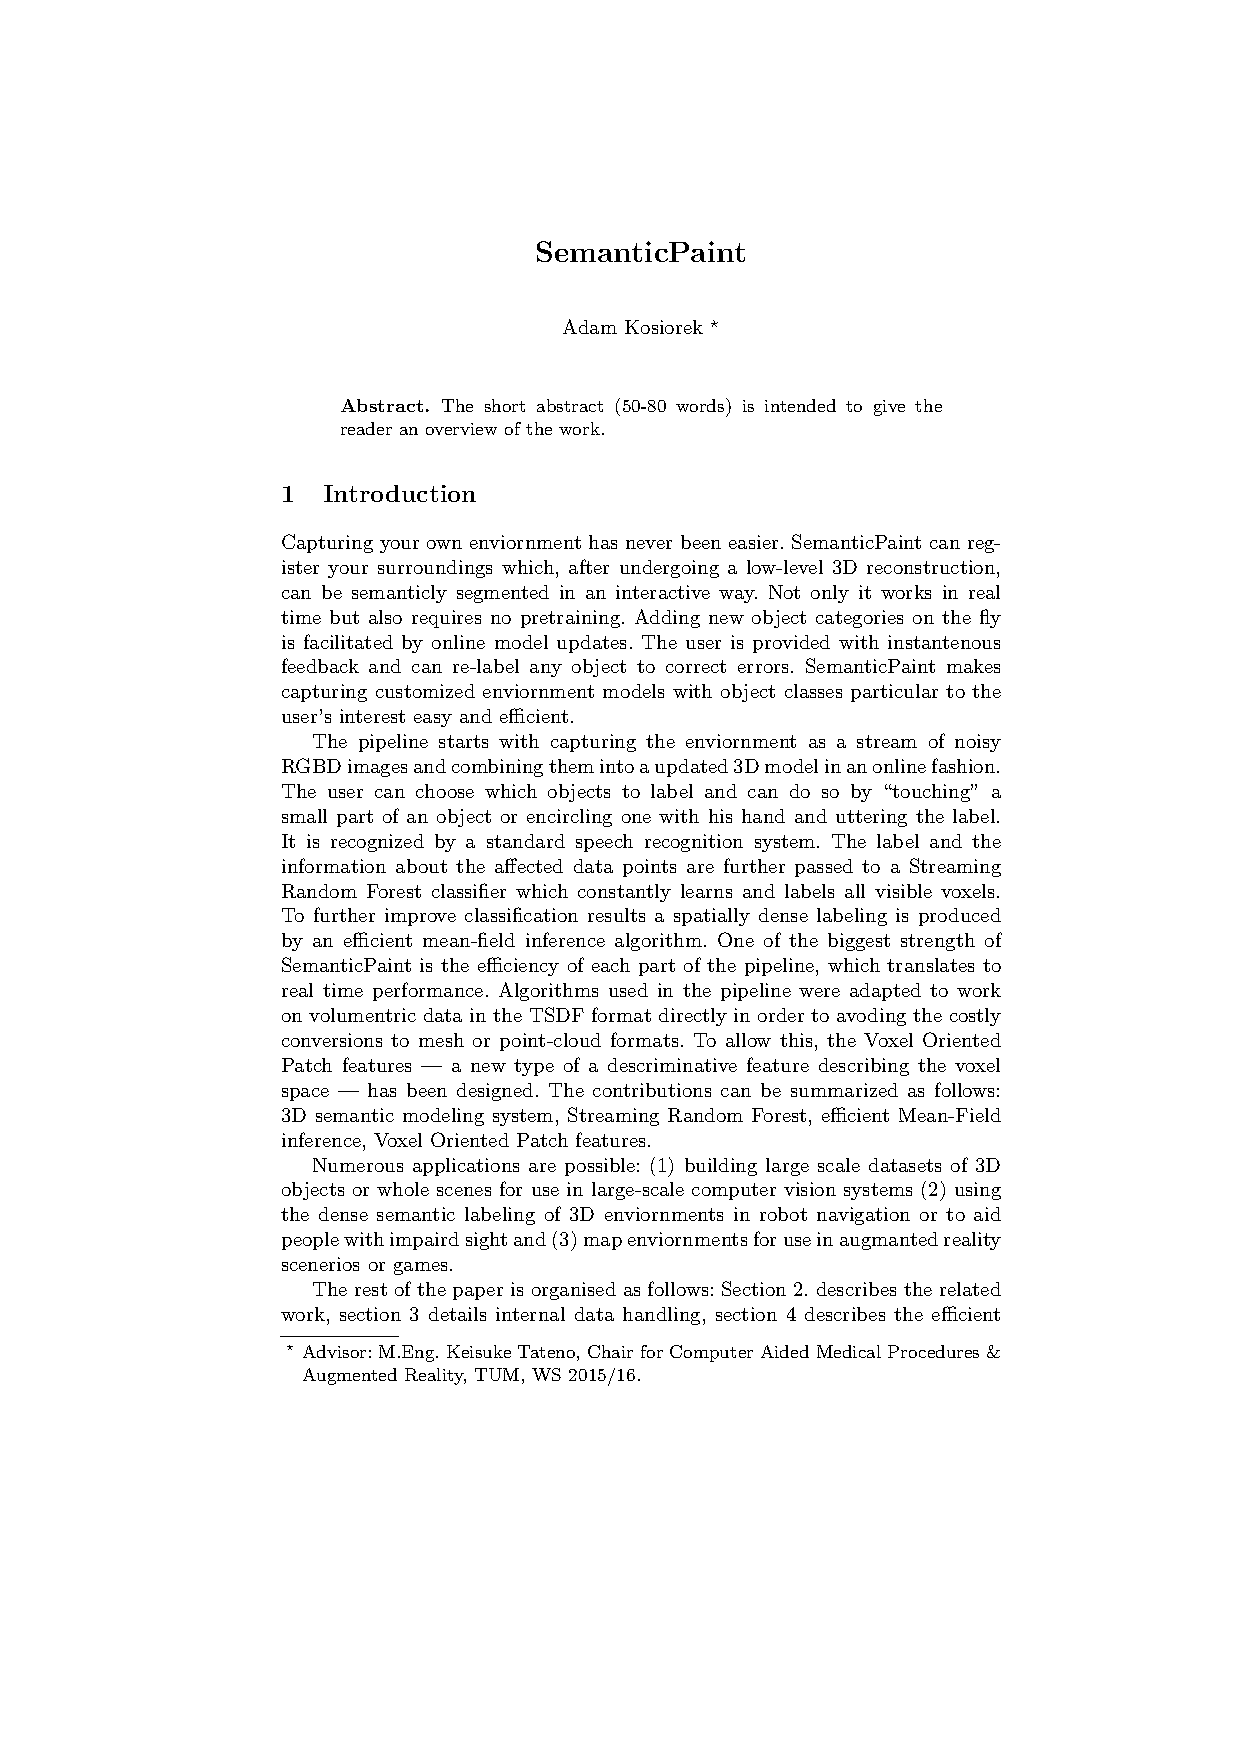
\includegraphics[height=\paperheight]{template}}

\setbeamertemplate{frametitle}{
	\vskip30pt
 	\usebeamercolor[blue!60!green]{frametitle}
  	\centering
  	\insertframetitle
	\vskip5pt
	\color{blue!60!green}{\hrule}
	}
}
\setbeamertemplate{footline}[frame number]
\setbeamercolor{math text}{fg=orange!80!black}
\newcommand{\hl}[1]{\textcolor{red!80!black}{\underline{#1}}}

\AtBeginSection[]{
  \begin{frame}
  \vfill
  \centering
  \begin{beamercolorbox}[sep=8pt,center,shadow=true,rounded=true]{title}
    \usebeamerfont{title}\insertsectionhead\par%
  \end{beamercolorbox}
  \vfill
  \end{frame}
}


\title[short title]{SemanticPaint}
\author[short presentator]{Adam Kosiorek}
\institute[CAMP]{Advisor: M.Eng.~Keisuke Tateno}
\date[]{10.12.2015}


\begin{document}

% 1. introduction
%   - lots of research in registration in visual understanding since the beginning of CV
%   - none approach so far achieved robust real time segmentation
%   - this paper introduces an end-to-end pipeline for interactive registration and segmentation of 3D enviornments
%   
% 2. State of the Art
%   - 
%   
% 3. Pipeline
%   - regristration and reconstruction
%   - classification
%   - crf and mean-field inference for smoothing
%   - VOPs
% 
%  4. Results
%   - dataset for segmentation and VOPs
%   - segmentation
%   - VOPs
%   - dataset for SRF
%   - SRF
%   
% 5. Discussion
%   - applications
%   - failures
%   
% 6. Summary
%   - what it is about
%   
% 7. Future Work
%   - scaling
%   - pure geometry
%   - (verbal) priors

%---------------------------------------------------------------------------------------

\begin{frame}
\titlepage
\pnote{name}
\pnote{framework for interactive capturing of 3D enviornments}
\end{frame}


%---------------------------------------------------------------------------------------

\begin{frame}{Outline}
\tableofcontents
\pnote{Let's start by seeing the framework in action}
\end{frame}



%---------------------------------------------------------------------------------------
\section{Introduction}

%---------------------------------------------------------------------------------------
\section{State of the Art}

\begin{frame}
\frametitle{Scene Understanding}

\begin{table}
\noindent\makebox[\linewidth]{
 \begin{tabular}{c|c|c}
  Who & What & How \\ \hline
  
  Valentin et. al. 2013  & inference on & RGB and geom. features  \\
  & mesh from TSDF  & CRF segmentation \\ \hline
    
  Kim et. al. 2013 & reconstruction & Voxel-based CRF \\ 
    & segmentation   & with visibility contraints\\ \hline
    
  Herbst et. al. 2014  & reconstruction & online model updates \\
     & segmentation & change detection\\ \hline
 \end{tabular}
}
\end{table}

\pnote{research on: RFB, D, point cloud, mesh, volume}
\pnote{most offline, not real time; CNN for class & detetect, CRF and variation for segm}
\pnote{Valentin}
\pnote{depth into volumetric TSDF, triangulated, mesh}
\pnote{rgb on img, geo on mesh}
\pnote{KITTI, NYU; mesh speed and accuracy}
\pnote{}
\pnote{Kim}
\pnote{voxel <- visibility and occupancy, vis constrained}
\pnote{model and reduce noise in depth maps}
\pnote{offline, global inference}
\pnote{}
\pnote{Herbst}
\pnote{detect change after model updates}
\pnote{static unchanged, dynamic changed}
\pnote{online but not real time, 2s per frame}

\end{frame}


\begin{frame}
\frametitle{Model-based SLAM}

\begin{table}
\noindent\makebox[\linewidth]{
 \begin{tabular}{c|c|c}
  Who & What & How \\ \hline
  Newcombe et. al. 2011  & online 3D SLAM & model-based tracking \\
  && global TSDF volume \\ \hline
  
  Salas-Moreno et al. 2013 & object-level & offline object database \\
  & SLAM & pose-object graph\\ \hline
  
  Pradeep et.al. 2013 & 3D reconstruction & sparse tracking and  \\
    & with 1 RGB camera  & stereo reconstruction \\
    && on par with KinectFusion
 \end{tabular}
}
\end{table}
 
\pnote{SLAM important in robotics, SemanticPaint relies heavily}
\pnote{major contribution by Newcombe, KinectFusion; 3D reconstruction from a single depth sensor}
\pnote{model-based tracking to match frame against model}
\pnote{global volume in TSDF}
\pnote{}
\pnote{extends KinectFusion -> object classification}
\pnote{match objects from the scene against a database}
\pnote{obj-pose graph, sparse, compact repr}
\pnote{sparse, requires offline database}
\pnote{}
\pnote{3D from single RGB camera}
\pnote{tracking, key and secondary frames, stereo reconsutrction}
\pnote{small scenes, good performance for textured}
\end{frame}

%---------------------------------------------------------------------------------------
\section{Pipeline}

\begin{frame}
\frametitle{Pipeline Overview}
\begin{figure}
 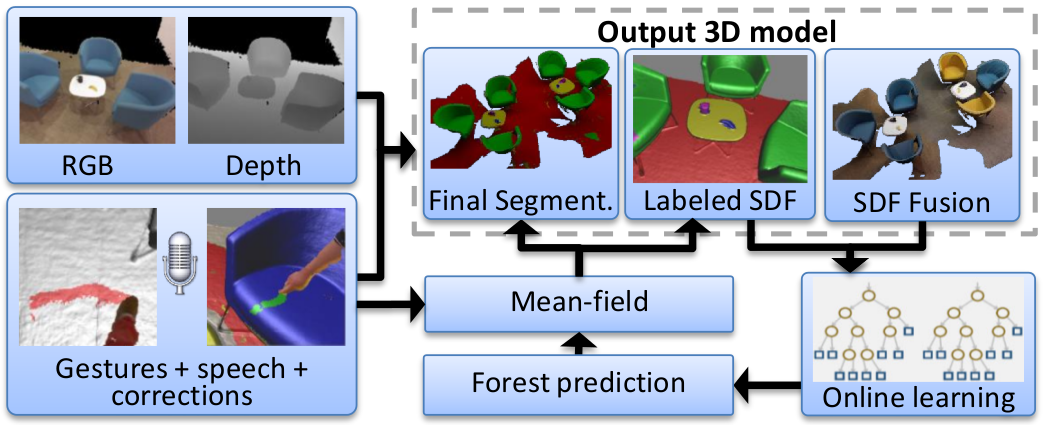
\includegraphics[width=\textwidth]{figures/pipeline}
\end{figure}

\pnote{depth + rgb = TSDF}
\pnote{user interactions = touched obj into CRF => priors}
\pnote{also into RF => predict labels for other objects}
\pnote{feedback loop: CRF gives labels from SRF, RF is trained on CRF}
\end{frame}

\begin{frame}
\frametitle{Voxel Oriented Patch features}

\begin{columns}
 \begin{column}{0.5\textwidth}
  \begin{figure}
  \center
  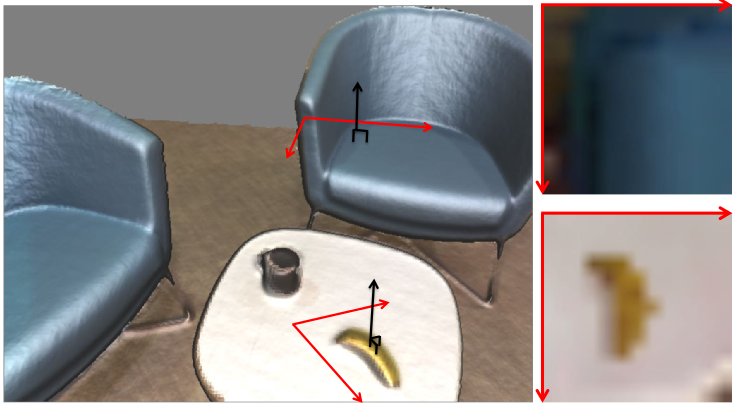
\includegraphics[width=\textwidth]{figures/vop}
  \caption{Colours shown in RGB for illustration purposes.}
  \label{fig:vop}
\end{figure}
 \end{column}
 \begin{column}{0.5\textwidth}
    $(\mathbf{p} - \mathbf{p}_i) \cdot \mathbf(n)_i = 0$ \\
    $r \times r$, $r = 13px$ with $10\frac{mm}{pixel}$\\
    CIELab\\
    Rotated to dominant gradient direction
 \end{column}
\end{columns}


\end{frame}

\begin{frame}
\frametitle{Random Forest}

\begin{columns}
 \begin{column}{0.5\textwidth}
  \begin{figure}
  \center
  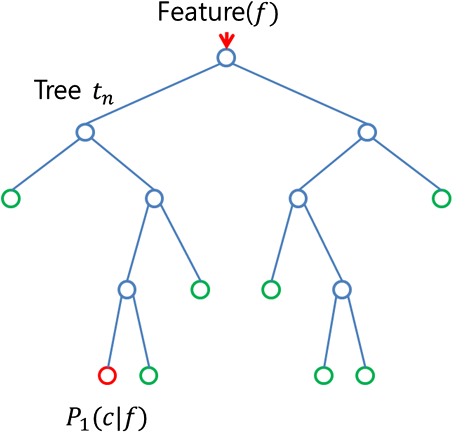
\includegraphics[width=\textwidth]{figures/rf}
  \caption{Single tree}
\end{figure}
 \end{column}
 \begin{column}{0.5\textwidth}
    bagged trees\\
    greedy training\\
    bootstraped data\\    
    off-line, all data at once\\
    voting for final result\\    
    
    $(i, l) \in \mathcal{S}$ - (voxel, label) pairs\\
    $f(i, \theta)$ - split functions\\
    $\Theta$ - distribution of split functions\\
    $P_F(x_i = l | \mathbf{D})$ - class conditional probability\\
 \end{column}

\end{columns}
\end{frame}

\begin{frame}
\frametitle{Streaming Random Forest}
  \begin{itemize}
   \item Node n: Reservoir $R_n$ with a list of samples $T_n$, $|T_n| \leq K$
   \item First $K$ samples added
   \item Current samples swapped with new ones with decreasing probability
   \item Split node if: $|R_n| > N$
  \end{itemize}

  Information Gain:
  \vspace{-0.25cm}
  \begin{equation} \label{eq:infogain}
    G(R_n, R_n^L, R_n^R) = H(R_n) - \sum_{d \in \{L, R\}} \frac{|R_n^d|}{|R_n|}H(R_n^d)
  \end{equation}
  Shannon Entropy:
  \vspace{-0.25cm}
  \begin{equation}
   H(R_n) = - \sum_{(l, i) \in T_n} p(c_i = l) \log{p(c_i = l)}
  \end{equation}
  
  \vspace{-0.25cm}
  $H(R_n)$ computed from a node's class distribution
  
  \pnote{SRF inherently online; some terminology}
  \pnote{the behind the reservoir: samples over huge time window -> unbiased sample of all data}
  \pnote{objective: Information Gain from normalized class distribution at each node}
\end{frame}

\begin{frame}
\frametitle{SRF - Reservoir Splitting}
$m_n$ - number of samples seen at node $n$\\
$P(l | T_n)$ - normalized class distribution of $R_n$
\vspace{-0.25cm}
\begin{figure}[!ht]
  \center
  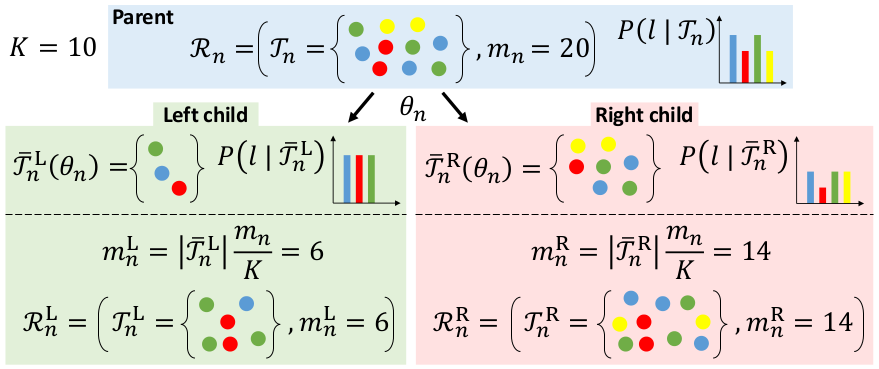
\includegraphics[width=\textwidth]{figures/forest}
%   \caption{Splitting reservoirs in Streaming Random Forest.}
  \label{fig:forest}
\end{figure}

\pnote{create node + distribution of split functions}
\pnote{split node -> sweep through R for every split function and compute class distributions}
\pnote{no explicit R computations are needed, just the splits}
\pnote{pass the statistics to child nodes}
\end{frame}

\begin{frame}
\frametitle{Dynamic Conditional Random Field}

Joint class probability distribution for the volume $\mathcal{V}$:
  \begin{equation} \label{eq:posterior}
  P(\mathbf{x}|\mathbf{D}) = \prod_{i \in \mathcal{V}} \left( \psi_i(x_i) \prod_{j \in \mathcal{E}_i} \psi_{ij}(x_i, x_j) \right) 
  \end{equation}

\vspace{-0.5cm}
Labeling Energy at time $t$:
  \begin{equation} \label{eq:energy}
  E_t(\mathbf{x}) = \sum_{i \in \mathcal{V}} \left( \phi_i(x_i) + \sum_{j \in \mathcal{E}_i} \phi_{ij} (x_i, x_j) \right) + K
  \end{equation}
  
\vspace{-0.5cm}  
where:\\
$\phi_i(x_i)$ - cost of assigning a label \\
$\phi_{ij}(x_i, x_j)$ - cost of assuming different labels\\
$\mathcal{E}_i$ - neighbourhood of voxel $i$

\pnote{CRFS subclass of PGMs; classification of sequences; global contex}
\pnote{in CV: segmentation; here: smoot out segm and user inter}
\pnote{}
\pnote{psi - likelihood and prior}
\pnote{distr -> NLL -> energy -> minimize}
\pnote{phi -> cost of label, smoothnes}
\pnote{eps -> neigbourhood, 6cm}
\end{frame}

\begin{frame}
\frametitle{CRF - User Interactions}

  Touching:
  \begin{columns}
   \begin{column}{0.25\textwidth}
    \begin{figure}
    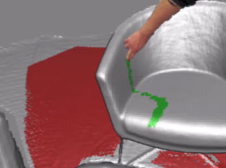
\includegraphics[width=\textwidth]{figures/touch}
    \end{figure}
    \end{column}
    \begin{column}{0.75\textwidth}
      \begin{equation}
	\phi_i(l) =
	  \begin{cases}
	    0      & \quad \text{if } l = l_T\\
	    \infty  & \quad \text{otherwise}\\
	  \end{cases}
      \end{equation}
      \center
      $T$ --- touched pixels
   \end{column}

  \end{columns}
  
  \vspace{0.5cm}
  Encircling:
  \vspace{-0.5cm}
    \begin{columns}
   \begin{column}{0.25\textwidth}
    \begin{figure}
    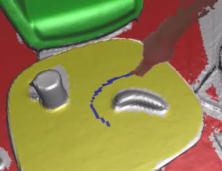
\includegraphics[width=\textwidth]{figures/circle}
    \end{figure}
   \end{column}
    \begin{column}{0.75\textwidth}
      \begin{equation}
  \phi_i(l) =
    \begin{cases}
      \log P_E(fg|\mathbf{a}_i)       & \quad \text{if } l = \text{fg}\\
      \log (1 - P_E(fg|\mathbf{a}_i))  & \quad \text{if } l = \text{bg}\\
    \end{cases}
  \end{equation}
  
  \center
  $P_E$ from GMM\\
  fg --- inside\\
  bg --- outside
   \end{column}
  \end{columns}

\pnote{Note -> changing energy landscape <- user interactions}
\pnote{touch and say -> set potentials; 0 if correct or inf otherwise}
\pnote{}
\pnote{circle more complication -> convex hull of selection as fg, others bg}
\pnote{fit GMM and infer in a boundix box around selection}
\pnote{to update potentials}
\end{frame}

\begin{frame}
\frametitle{CRF - Predictions and Smoothnes}

  Predictions:
  \begin{equation}
  \phi_i(l) = -\log P_F(x_i = l | \mathbf{D})
  \end{equation}
  $P_F$ --- Streaming Random Forest prediction

  \vspace{0.5cm}
  Smoothnes:
  \begin{equation}
      \phi_{ij}(x_i, x_j)  = \theta_p e^{-||\mathbf{p}_i - \mathbf{p}_j||}  + \theta_a e^{-||\mathbf{a}_i - \mathbf{a}_j||} + \theta_n e^{-||\mathbf{n}_i - \mathbf{n}_j||}
  \end{equation}
  
  $\theta_p$, $\theta_a$, $\theta_n$ --- paramters \\
  $\mathbf{p}_i$ --- position\\
  $\mathbf{a}_i$ --- appearance\\
  $\mathbf{n}_i$ --- normal vector
  
  
\pnote{Next come forest predictions -> update pot of otherwise unaffected voxels -> NLL of current class}
\pnote{smothness -> priors based on differences}
\end{frame}

\begin{frame}
\frametitle{Mean-Field Inference}
$P(\mathbf{x})$ approximated by $Q(\mathbf{x})$ under $KL(Q||P)$:
\begin{equation}
 Q_i^t(l) = \frac{1}{Z_i}e^{M_i(l)} \text{, } t = 1, \ldots, T
\end{equation}
\begin{equation}
 M_i(l) = \phi_i(l) + \sum_{l' \in \mathcal{L}} \sum_{j \in \mathcal{E}_i} Q_j^{t-1}(l')\phi_{ij}(l, l')
\end{equation}


Frame at time $t$ initialized with:
\begin{equation}
 \widetilde{Q}_i^t(x_i) = \gamma Q_i^{t-1}(x_i) + (1 - \gamma) P_F^{t-1}(x_i = l | \mathbf{D}) \text{, } \gamma \in [0, 1]
\end{equation}

\pnote{Then comes mean-field inference}
\pnote{approximate original P(x) under KL with Q(x)}
\pnote{iterative algo to refine}
\pnote{gradual change of energy landscape}
\pnote{single update in each frame}
\pnote{to speed up RF's impact -> initialization}
\end{frame}

%---------------------------------------------------------------------------------------
\section{Results}
\begin{frame}
\frametitle{Segmentation}
  \begin{figure}
   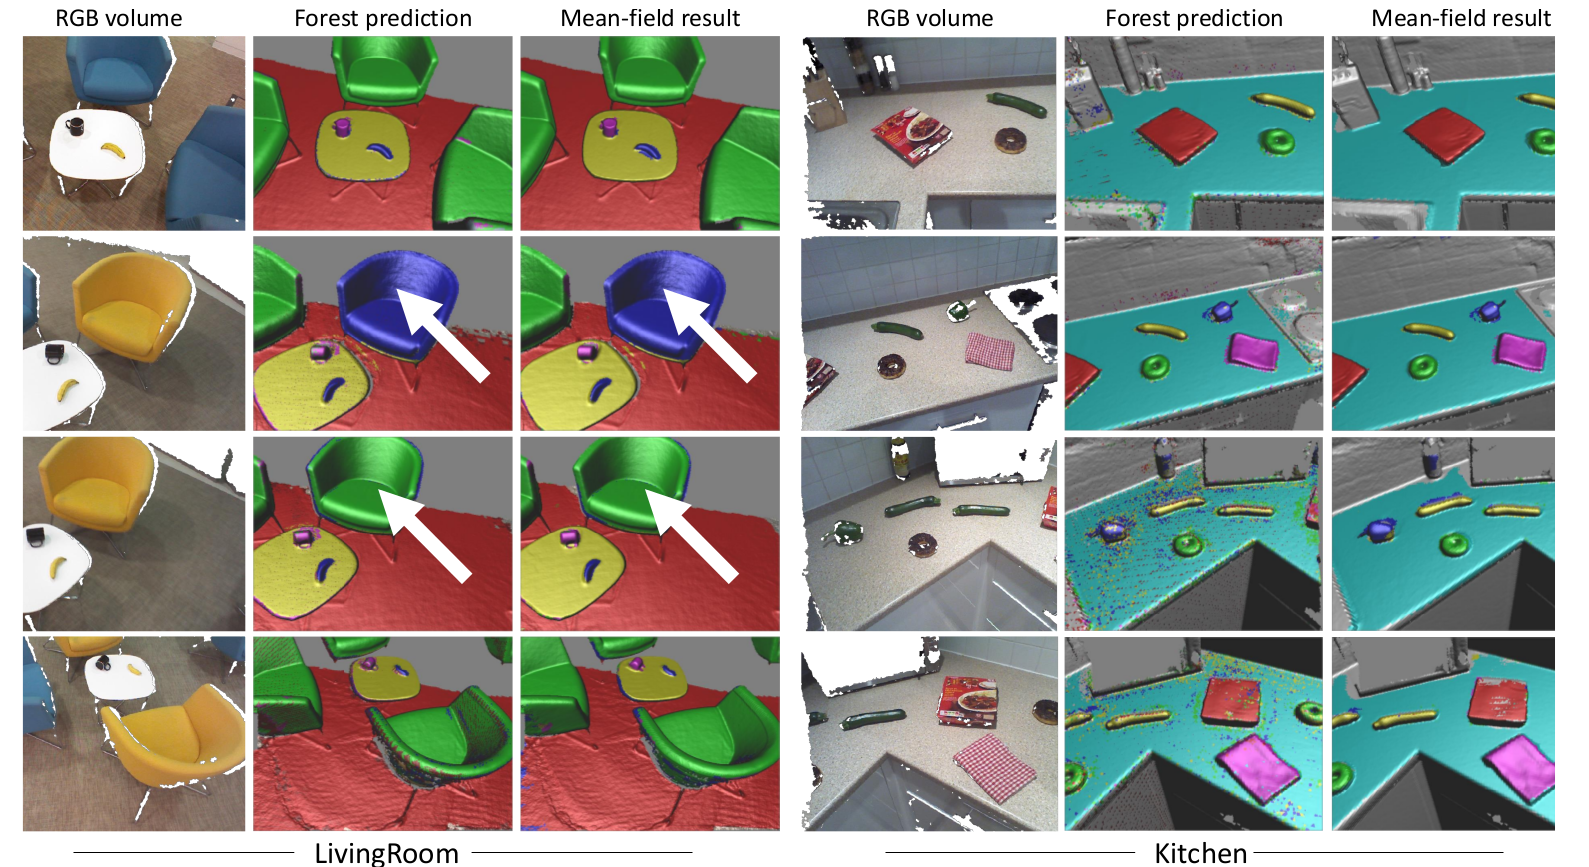
\includegraphics[width=\textwidth]{figures/results}
  \end{figure}

\pnote{Let's look at some segmentation results}
\pnote{We have... for 2 different scenes}
\pnote{inference improves results quite a lot}
\pnote{we can relabel and correct mistakes}
\end{frame}

\begin{frame}
\frametitle{Segmentation}

\begin{table}[!ht]
 \fontsize{10pt}{7.2}\selectfont
 \center
 \caption{Segmentation Results}
\noindent\makebox[\linewidth]{
  \begin{tabular}{c|c|c|c|c|c}
    \textbf{Component} & \textbf{LivingRoom} & \textbf{Bedroom} & \textbf{Kitchen} & \textbf{Desk} & \textbf{Average} \\ \hline
    User Interaction & 99.35\% & 97.61\% & 96.09\% & 97.73\% & 97.7\% \\ 
    Forest Prediction & 94.57\% & 88.31\% & 82.58\% & 90.29\% & 88.94\% \\
    Final Inference & 96.26\% & 95.19\% & 90.69\% & 95.55\% & 94.42\%
  \end{tabular}
 }
 \label{fig:segm_results}
\end{table}


\pnote{if we look at percentage}
\pnote{iteraction very well}
\pnote{RF ok}
\pnote{mean-field smoothing improves}
\end{frame}

\begin{frame}
\frametitle{Features}
\vspace{-0.25cm}
 \begin{figure}[!ht]
  \center
  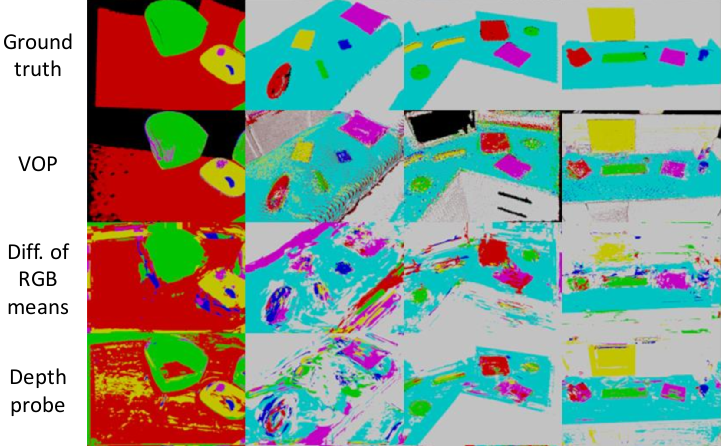
\includegraphics[width=\textwidth]{figures/results_vop}
%   \caption{Average Precision}
%   \label{fig:srf_ap}
  \end{figure}
  
\pnote{Next, let's look at features}
\pnote{compared indirectly by comparing how RF behaves while using different features}
\pnote{discriminative power}
\pnote{here: 3 best results; VOP most consistent}

\end{frame}

\begin{frame}
\frametitle{Features}

\begin{table}[!ht]
 \fontsize{10pt}{7.2}\selectfont
 \center
 \caption{Feature Comparison}
 \noindent\makebox[\linewidth]{
  \begin{tabular}{c|c|c|c|c|c}
  \textbf{Feature} & \textbf{LivingRoom} & \textbf{Bedroom} & \textbf{Kitchen} & \textbf{Desk} & \textbf{Average} \\ \hline
  VOP & \textbf{94.57\%} & \textbf{88.31\%} & 82.58\% & \textbf{90.29\%} & \textbf{88.94\%} \\
  $\Delta$ RGB mean & 80\% & 71.84\% & 76.29\% & 73.42\% & 75.39\% \\
  Depth Probe& 77.54\% & 61.79\% & \textbf{84.9\%} & 68.9\% & 73.06\% \\
  Color Probe& 56.39\% & 65.68\% & 60.77\% & 60.74\% & 60.9\% \\
  SURF & 43.74\% & 67.12\% & 57\% & 58.13\% & 56.5\% \\
  SPIN & 58.77\% & 43.22\% & 48.41\% & 36.1\% & 46.63\% \\
 \end{tabular}
 }
 \label{fig:vop_results}
\end{table}

\pnote{Again, if we look at percentage, VOP the best}
\pnote{Kitchen is worse -> harsh illumination}
\pnote{makes RGB feature inconclusive}
\end{frame}

\begin{frame}
\frametitle{Streaming Random Forest}

\begin{columns}
 \begin{column}{0.5\textwidth}
  \begin{figure}[!ht]
  \center
  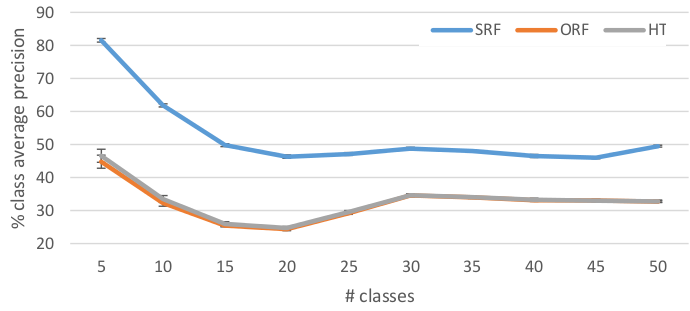
\includegraphics[width=\textwidth]{figures/srf_ap}
  \vspace{-0.25cm}
  \caption{Average Precision}
  \label{fig:srf_ap}
  \end{figure}
  \vspace{-0.5cm}
  \begin{figure}[!ht]
  \center
  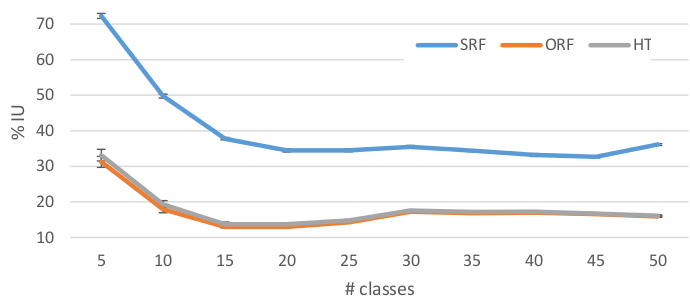
\includegraphics[width=\textwidth]{figures/srf_iu}
  \vspace{-0.25cm}
  \caption{Intersection/Union}
  \label{fig:srf_iu}
  \end{figure}
 \end{column}
 
 \begin{column}{0.5\textwidth}
  Data:\\
  300 objects\\
  51 classes\\
  full revolution\\
  3 points of view \\
  \vspace{0.5cm}
  SRF - Streaming Random Forest\\
  ORF - Online Random Forest\\
  HT - Hoeffding Tree \\
 \end{column}
\end{columns}

\pnote{SRF against two other tree-based online classifiers ORF and HT}
\pnote{simulate online setting: add new classes and PoVs sequentially}
\pnote{SRF outperforms comfortably, more effiiicient}
\pnote{Sad fact: accurayc drops with classes}
\pnote{handling coplicated scenes tricky}
\end{frame}


%---------------------------------------------------------------------------------------
\section{Discussion and Outlook}
\begin{frame}
\frametitle{Summary}
\begin{itemize}
 \item customized models of 3D enviornments
 \item fully interactive
 \item online and real time
 \item no pretraining
\end{itemize}

\pnote{To sum up: delivers pipeline that lets capture personalized 3D envs as you need}
\pnote{fully interactive, req no pretrain and works online}
\pnote{possible apps: robot navi, sighted people, datasets for large-scale CV}
\end{frame}

\begin{frame}
\frametitle{Failures}
\begin{columns}
 \begin{column}{0.5\textwidth}
  \begin{figure}[!ht]	 
  \center
  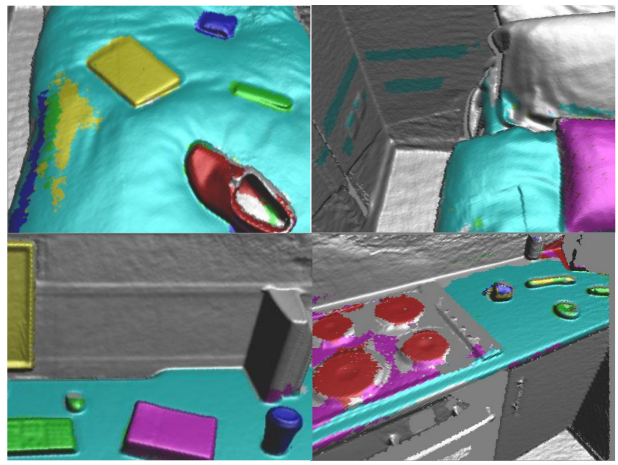
\includegraphics[width=\textwidth]{figures/failures}
  \caption{Failure cases.}
  \label{fig:failures}
  \end{figure}
 \end{column}
 
 \begin{column}{0.5\textwidth}
  \begin{itemize}
   \item bleeding
   \item illumination change
   \item viewpoint change
  \end{itemize}
 \end{column}
\end{columns}

\pnote{Unf, some failures}
\pnote{Bleeding, or misclassif at object edges <- errors of depth and colour sensor alignm}
\pnote{big illumination and viewpoint changes -> errors}
\end{frame}

\begin{frame}
\frametitle{Future Work}
\begin{itemize}
  \item discriminative geometrical features
  \item priors for class properties (vertical walls)
 \item class priors for different enviornments
 \item outdoor enviornments
 \item better scalability
\end{itemize}

\pnote{Some future work to be done}
\pnote{Geo features -> prevent bleeding}
\pnote{class priors (vertical walls) and for diff envs -> better accuracy}
\pnote{outdoor envs -> passive sensors}
\pnote{bigger scenes and more classes -> scalable algos}
\end{frame}


%---------------------------------------------------------------------------------------
\begin{frame}
\frametitle{References}
\fontsize{6pt}{7.2}\selectfont
\begin{itemize}
  \item Roberts, L. G. 1963. Machine perception of three-dimensional solids. Ph.D. thesis, Massachusetts Institute of Technology.

  \item Kim, B.-S. et. al. 2013. 3D scene understanding by voxel-CRF. In Proc. ICCV.

  \item Pradeep, V. et. al. 2013. Monofusion: Real-time 3D reconstruction of small scenes with a single web camera. In Proc. ISMAR.

  \item Herbst, E. et.al. 2014. Toward online 3-d object segmentation and mapping. In IEEE International Conference on Robotics and Automation (ICRA).

  \item Valentin, J. P. et. al. 2013. Mesh based semantic modelling for indoor and outdoor scenes. In Proc. CVPR.

  \item Salas-Moreno, R. F. et. al. 2013. SLAM++: Simultaneous localisation and mapping at the level of objects. In Proc. CVPR.

  \item Newcombe , R. A. et. al. 2011. KinectFusion: Real-time dense surface mapping and tracking. In Proc. ISMAR.  
  
  \item Curless , B. et. al. 1996. A volumetric method for building complex models from range images. In Proceedings of the 23rd annual conference on Computer graphics and interactive techniques. ACM, 303–312.
  
  \item Niessner , M. et. al. 2013. Real-time 3D reconstruction at scale using voxel hashing. ACM TOG 32, 6
\end{itemize}
\end{frame}


%---------------------------------------------------------------------------------------
\begin{frame}
\frametitle{References cont'd}
\fontsize{6pt}{7.2}\selectfont
\begin{itemize}
  \item Saffari , A. et. al. 2009. On-line random forests. In IEEE ICCV Workshop.
  
  \item Vitter , J. S. 1985. Random sampling with a reservoir. ACM TOMS 11, 1. 
  
  \item Lower , D. G. 1999. Object recognition from local scale-invariant features. In Proc. ICCV.
  
  \item Lafferty , J. et. al. 2001. Conditional random fields: Probabilistic models for segmenting and labeling sequence data.
  
  \item Ktahenbül, P. et. al. 2011. Efficient inference in fully connected CRFs with Gaussian edge potentials. In NIPS.

  \item Koller , D. et.al  , N. 2009. Probabilistic Graphical Models: Principles and Techniques. MIT Press
  
  \item Domingos, P. et. al. 2000. Mining high-speed data streams. In Proc. SIGKDD.
	
  \item Lai, K. et. al. 2011. A large-scale hierarchical multi-view rgb-d object dataset. In Proc. ICRA.
  
  \item Valentin, J. et. al. 2015. SemanticPaint: Interactive 3D Labeling and Learning at your Fingertips. SIGGRAPH.
\end{itemize}
\end{frame}

\begin{frame}
\frametitle{Q\&A?}
\begin{figure}
 \includegraphics[width=0.8\textwidth]{figures/SemanticPaint}
\end{figure}

\end{frame}


%---------------------------------------------------------------------------------------
\end{document}



